\graphicspath{{chapter4/figures/}}
\chapter{Automatic pulmonary function estimation from chest CT scans using deep regression neural networks: the relation between structure and function in systemic sclerosis}
\label{chap:4}

% This is for title at the border of the page
\runningchaptertitle{PFT estimation from CT}

% This is an example to put the publication
\publishedat{}{\textbf{Jia, J.}, Zhai, Z., Bakker, M. E., Hernández-Girón, I., Staring, M., \& Stoel, B. C. (2021, April). \textbf{Multi-task semi-supervised learning for pulmonary lobe segmentation}. In \textit{2021 IEEE 18th International Symposium on Biomedical Imaging (ISBI) }(pp. 1329-1332). IEEE.} 

\ThumbIndexShow
%---------------------------------------

\begin{abstract}
% \section{Abstract} 
Pulmonary function tests (PFTs) play an important role in screening and following-up pulmonary involvement in systemic sclerosis (SSc). However, some patients are not able to perform PFTs due to contraindications. In addition, it is unclear how lung function is affected by changes in lung structure in SSc. Therefore, this study aims to explore the potential of automatically estimating PFT results from chest CT scans of SSc patients and how different regions influence the estimation of PFTs. Deep regression networks were developed with transfer learning to estimate PFTs from 316 SSc patients. Segmented lungs and vessels were used to mask the CT images to train the network with different inputs: from entire CT scan, lungs-only to vessels-only. The network trained on entire CT scans with transfer learning achieved an ICC of 0.71, 0.76, 0.80, and 0.81 for the estimation of DLCO, FEV\textsubscript{1}, FVC and TLC, respectively. The performance of the networks gradually decreased when trained on data from lungs-only and vessels-only. Regression attention maps showed that regions close to large vessels were highlighted more than other regions, and occasionally regions outside the lungs were highlighted. These experiments show that apart from the lungs and large vessels, other regions contribute to PFT estimation. In addition, adding manually designed biomarkers increased the correlation (R) from 0.75, 0.74, 0.82, and 0.83 to 0.81, 0.83, 0.88, and 0.90, respectively. This suggests that that manually designed imaging biomarkers can still contribute to explaining the relation between lung function and structure.
\end{abstract}
\clearpage

\section{Introduction}
Systemic sclerosis (SSc) is a rare immune-mediated connective tissue disease that affects different organs. Interstitial lung disease (ILD) is, however, the leading cause of morbidity and mortality, and up to 90\% of SSc patients have pulmonary function abnormalities \cite{Behr2008}. To evaluate progression of SSc-ILD, various pulmonary function tests (PFTs) are used as key measures, such as the diffusion capacity for carbon monoxide (DLCO), forced expiratory volume in 1 second (FEV\textsubscript{1}), forced vital capacity (FVC) and total lung capacity (TLC) \cite{Behr2008, Caron2018, Ninaber2015}. In clinical practice, PFTs are expressed either in absolute values or in percent predicted values (abbreviated as PFTs\%pred, including DLCO\%pred, FEV\textsubscript{1}\%pred, FVC\%pred and TLC\%pred). PFTs\%pred are obtained by the standardization of the absolute values according to the patients’ characteristics to avoid biases from sex, ethnicity and height \cite{Graham2019}. A PFT\%pred below 100\% then represents a lung function that is lower than the average lung function in a population with the same age, gender, etc., with upper and lower limits of normal (usually 1.64 SD). Both absolute and percent predicted are commonly used clinically as outcome measures for progression of SSc-ILD \cite{Caron2018}. 

PFTs can, however, not always be performed if there is a risk of disease transmission, e.g. in patients with COVID-19, active tuberculosis or other airborne infectious diseases \cite{choi2022automated, McGowan2022}. In addition, some patients, who have hemoptysis or had surgery in the past month, or other contraindications \cite{Cooper, Meng2023}, like aneurysmatic abnormalities and ischaemic stroke, are not able to perform PFTs because the forced exhalation during spirometry may increase the risk of complications [9]. Therefore, alternative methods to estimate PFT are of great interest. Because CT could provide high-resolution details of the lungs, it is regarded the gold standard for diagnosing SSc-ILD \cite{Sylvester2020}. In previous research, quantitative biomarkers have been extracted from chest CT images of SSc patients, which correlate with PFTs [11???]. Therefore, when PFTs are not possible and CT scans have been made for SSc patients, it is of great interest to see if CT could be used to estimate PFT.

Apart from being an alternative to PFTs, PFT estimation from CT scans can also be used to study the relation between structure and function as the lungs become affected by SSc-ILD. Initially, imaging biomarkers were designed for SSc to explicitly describe lung structure and subsequently determine their correlation with lung function. For SSc patients with fibrosis, Goh \textit{et al}. \cite{Goh2007} designed a visual fibrosis scoring system, which correlated with FVC (R = -0.40). For SSc patients without fibrosis visible on CT, Zhai \textit{et al}. \cite{Zhai2019} found that two vascular tree-based biomarkers ($\alpha$ and $\beta$) , which represent the lung vessel radius histogram, correlated with DLCO\%pred (R=-0.29 and 0.32, respectively). For SSc patients with or without fibrosis, Ninaber \textit{et al}. \cite{Ninaber2015} found that lung density, measured by the 85\textsuperscript{th} percentile density (Perc85) from CT scans, correlated significantly with DLCO\%pred (R=-0.49) and FVC \%predicted (R=-0.64). 

Apart from these manually designed biomarkers, an altogether different approach would be to develop a deep learning model that is trained to output PFT prediction values directly, with or without fibrosis visible on CT scans. Subsequently, the trained model could be studied in detail to explore the relation between lung structure from CT and lung function from PFTs.

To the best of our knowledge, we are the first to estimate PFTs for SSc patients. There are no works to estimate PFTs for SSc patients previously. The most relevant and recent works on automatic estimation of PFTs from chest CT using deep learning \cite{choi2022automated, Park2023} are not for SSc patients. Choi, \textit{et al}. \cite{choi2022automated} developed a network to estimate FEV\textsubscript{1} and FVC for patients before their first lung cancer surgery. Their network consisted of a ResNet-50 for feature extraction and a bidirectional long short-term memory (BiLSTM) network for PFT prediction. Park, \textit{et al}. \cite{Park2023} trained two separate I3D networks to estimate FEV\textsubscript{1} and FVC, respectively, for subjects at risk of lung cancer. It is unclear if their models could be applied directly to SSc patients. In addition, both methods estimate FEV\textsubscript{1} and FVC only, lacking DLCO and TLC. For determining SSc-ILD progression, however, TLC and especially DLCO are important measurements, the latter of which is most predictive of adverse outcomes, including death \cite{Caron2018}. Therefore, the aim of this study was to 1) develop a deep learning model to estimate DLCO, FEV\textsubscript{1}, FVC and TLC for SSc patients from their CT scans; and 2) explore the contribution of different anatomical regions, and provide explanations from a clinical perspective.

The remaining paper is organized as follows. Section 2 describes the datasets and methods we used for the prediction of PFT. Detailed experiments and results are shown in Section 3. Finally, section 4 discusses the experiments, explains the results and concludes the paper.


\section{Materials and methods}
\subsection{Dataset}
In this study, we retrospectively selected 333 patients who were referred to our targeted outpatient health care program (combined care in systemic sclerosis) between April 2009 and October 2015 in Leiden University Medical Center. Because of the diagnosis of SSc according to the referring rheumatologist, or a strong suspicion for SSc, they underwent high-resolution CT scans, followed by pulmonary function tests. As shown in Figure \ref{fig:chap4_flowchart}, we excluded seven patients with a CT-PFT interval greater than ten days, nine patients with incomplete PFTs, and one patient with a low-quality CT scan, resulting in 316 CT-PFT pairs. The dataset was split into two disjoint groups: 252 for four-fold training and cross-validation, and 64 for testing. The research protocol was granted approval by the local Medical Ethics Committee and written informed consent was provided by all patients.


\begin{figure}[tb]
    \centering
    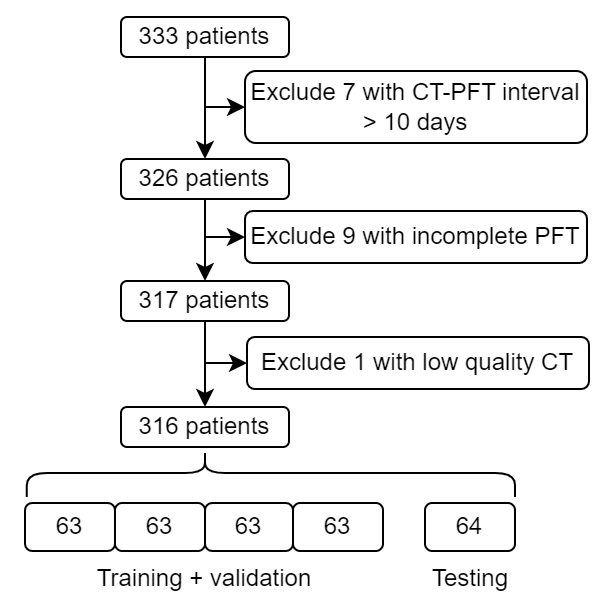
\includegraphics[width=8cm]{flowchart.png}
    \caption{Flowchart of the dataset inclusion and partition.}
    \label{fig:chap4_flowchart}
\end{figure}

% Please add the following required packages to your document preamble:
% \usepackage[table,xcdraw]{xcolor}
% If you use beamer only pass "xcolor=table" option, i.e. \documentclass[xcolor=table]{beamer}
\begin{table}[tb]
\centering
\caption{Dataset characteristics}
\begin{tabular}{lc}
\hline
Characteristic                                & Patients   (n=316) \\ \hline
Age, mean  ±  standard deviation {[}years{]}    & 53.4 ± 14.6        \\
Female (\%)                                   & 258 (81.4)         \\
Interstitial lung disease detected on CT (\%) &                    \\
Anti-centromere antibodies positive (\%)      &                    \\
Anti-topoisomerase antibodies positive (\%)   &                    \\
Pulmonary arterial hypertension (\%)          &                    \\
Disease Subset:                               &                    \\
\quad Non-cutaneous (\%)                            &                    \\
\quad Diffuse cutaneous (\%)                        &                    \\
\quad Limited cutaneous (\%)                        &                    \\
\quad Alternative diagnosis* (\%)                   &                    \\
Pulmonary Function, Mean ± Std                &                    \\
\quad DLCOc, {[}mL/min/mm Hg{]}                    & 5.55 ± 1.92        \\
\quad FEV\textsubscript{1}, {[}L{]}                                 & 2.62 ± 0.77        \\
\quad FVC, {[}L{]}                                  & 3.32 ± 0.97        \\
\quad TLC, {[}L{]}                                  & 4.91 ± 1.23        \\
\quad DLCOc\%, {[}\%{]}                            & 71.95 ± 20.10      \\
\quad FEV\textsubscript{1}\%, {[}\%{]}                             & 89.32 ± 17.69      \\
\quad FVC\%, {[}\%{]}                              & 90.58 ± 18.97      \\
\quad TLC\%, {[}\%{]}                              & 85.62 ± 17.07     \\ \hline
\end{tabular}
\label{chap4_table: dataset}
\end{table}




\textbf{CT scanning.} All subjects underwent scanning at full inspiration without contrast enhancement using an Aquilion 64 CT scanner (Canon Medical Systems), configured at 120 kVp, a median tube current of 140 mA, a rotation time of 0.4 seconds, a collimation of 64 × 0.5 mm and a helical beam pitch of 0.8; leading to a median CTDI\textsubscript{vol} of 8.2 mGy. The images were reconstructed with filtered back projection and an FC86 kernel, with a median pixel spacing of 0.64 mm × 0.64 mm, with a slice thickness and increment of 0.5 and 0.3 mm, respectively.

\textbf{PFT measurements.} PFTs were performed by an experienced technologist using a spirometer under ERS/ATS guidelines \cite{Miller2005, Graham2017} including single-breath diffusion capacity for carbon monoxide corrected for haemoglobin concentration (DLCO), forced expiratory volume in 1 second (FEV\textsubscript{1}), forced vital capacity (FVC) and total lung capacity (TLC). While DLCO was measured in units of mm/Hg/min, FEV\textsubscript{1}, FVC, TLC were measured in units of liter. The PFT percent predicted values (PFTs\%pred) were calculated with the latest official conversion equations and reference values \cite{Hall2021, Stanojevic2017, Quanjer2012}. Clinical characteristics of the 316 patients are shown in Table \ref{chap4_table: dataset}.

\begin{figure}[tb]
    \centering
    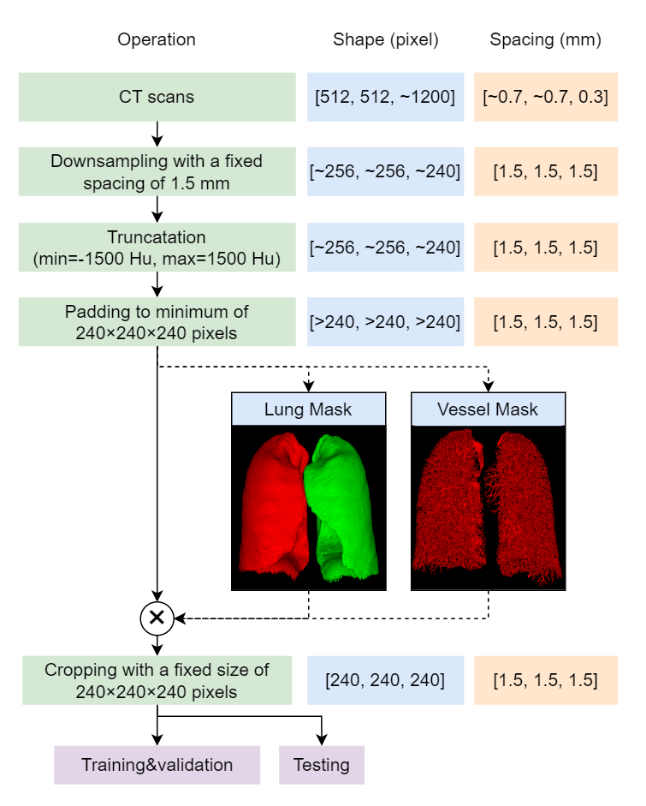
\includegraphics[width=8cm]{preprocessing.png}
    \caption{CT scan preprocessing procedure.}
    \label{fig:chap4_preprocessing}
\end{figure}

\textbf{Data preprocessing and augmentation.} Because of GPU memory limitations, we first down-sampled all CT scans to an isotropic spacing of 1.5 mm, as illustrated in Figure \ref{fig:chap4_preprocessing}, resulting in a median image size of 256 × 256 × 240 voxels. Next, we performed intensity truncation to clip voxel values between -1500 and 1500 HU to remove some artifacts. Then we applied padding, if necessary, to guarantee a minimum image size of 240 × 240 × 240 voxels. To subsequently augment the training data, a random 3D patch of a fixed size (240 × 240 × 240 voxels, which was ensured to cover the whole lung area) were cropped from each volume as they are fed into the model. In different epochs, different 3D patches were cropped from each CT for training. The epoch number is the number of 3D patches cropped from each CT. In the validation and testing phase, we used 3D patches of 240 × 240 × 240 voxels at the center position, from (\textit{x}0-120, \textit{y}0-120, \textit{z}0-120) to (\textit{x}0+120, \textit{y}0+120, \textit{z}0+120) where (\textit{x}0, \textit{y}0, \textit{z}0) is the coordinates of the center point of each validation and testing CT image. To investigate the contribution of different chest regions, we masked the CT images using various masks. Lung masks were obtained by a multi-atlas based method \cite{Zhai2019}, while vessel masks were acquired using a graph-cut based vessel segmentation network \cite{zhai2016lung}. The segmentation of lung and vessel masks was obtained by an in-house script in MeVisLab 2.7.1 (VC12-64). The implementation details could be found at the online document which were released along with the original paper \cite{Zhai2016} (http://links.lww. com/JTI/A114). The source code of our in-house script for the segmentation could be found at https://github.com/Zhiwei-Zhai/Lung-Vessel-Segmentation-Using-Graph-cuts. No additional data augmentation was performed.


\subsection{Network design}
The network was adapted from X3D \cite{Feichtenhofer}, which was originally designed for video recognition. The original paper proposed a series of networks with different capacities. An X3D of medium size (X3D-M) was selected as the architecture of our network, to account for limited GPU memory. As illustrated in Figure \ref{fig:chap4_x3d}, the network consists of several convolution and max-pooling layers, followed by four ResNet blocks with max-pooling layers between each of them, and finally one global average-pooling layer (GAP) and two fully connected (FC) layers. The output of the last FC layer has four values, representing the four (absolute) PFT parameters, simultaneously estimated in one network. We also developed four separate networks with 1-class outputs for each of them, estimating the different PFT parameters, separately. The comparison between these 1-class and 4-class networks will be shown later in Q4 of Section Experiments and Results.

\begin{figure}[tb]
    \centering
    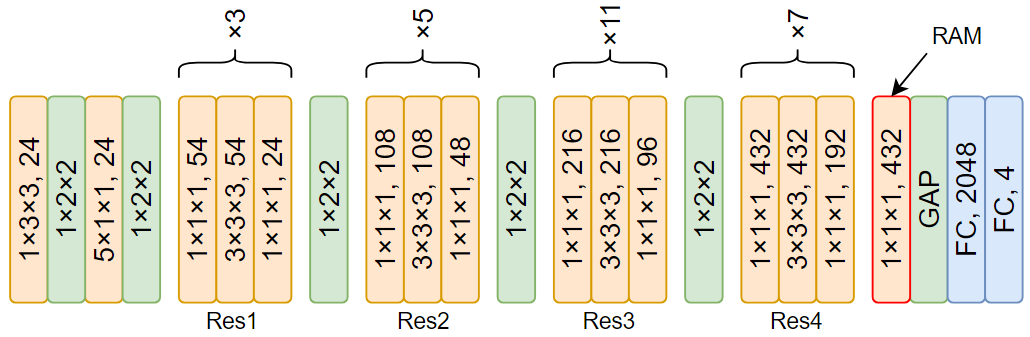
\includegraphics[width=8cm]{x3d.png}
    \caption{X3D-M structure. The whole network consists of 3D convolution layers (orange boxes), max-pooling layer (green boxes) and two fully connected layer (blue box). Kernel size (xyz) and channel number are denoted by the first three numbers and the last number, respectively.}
    \label{fig:chap4_x3d}
\end{figure}

To increase network performance, we introduced transfer learning (TL), in which the network was initialized by the weights trained from another domain. Although it may achieve better performance if the source domain is similar with the target domain, the lack of large annotated lung CT dataset makes it impractical to apply pre-trained weights from lung CT dataset. However, TL has been widely used in deep learning because it was reported to improve network performance significantly even if the source domain is different \cite{Cheplygina2019}. Therefore, our X3D-M network was pre-trained on Kinetics, a human action video dataset \cite{Feichtenhofer, Kay} (pytorch.org/hub/facebookresearch\_pytorchvideo\_x3d). Although there are other 3D networks which may also works on our task, X3D-M is the network which was released recently, achieved the SOTA performance, publish their pre-trained weights from Kinetics dataset, and could be fit into our GPU with memory of 11 GB.

We studied two ways to estimate PFTs\%pred: 1) directly, by one network that is trained to estimate PFTs\%pred directly; and 2) indirectly, where the absolute PFTs are obtained by a network, from which the PFTs\%pred are subsequently calculated by the official conversion equations \cite{Hall2021, Stanojevic2017, Quanjer2012}.


\subsection{Relation between lung structure and function}
After we obtained the optimized network and training method, we performed two strategies to understand how the network derived the estimation and how each chest region (such as muscle, lung, vessel, etc.) contributed to the PFT estimation. The first strategy was to train multiple networks with various inputs: whole CT image, lungs-only (by excluding the volume outside the lungs), left or right lung-only, vessels-only and the binarized version of vessels-only. The difference in performance between the different networks implies the contribution of these different regions. The second strategy was 3D regression activation mapping (RAM-3D), which is a variant of the Grad-CAM  \cite{Selvaraju} on 3D regression tasks. The original Grad-CAM was designed for 2D image classification \cite{Selvaraju}, which could generate heat maps to highlight the important regions for classification by convolutional neural networks (CNNs). Inspired by that, Wang \textit{et al}. proposed a RAM for 2D image regression \cite{wang2017diabetic}. In this work, we extended this RAM from 2D to 3D to highlight areas of interest in the 3D CT volumes for the PFT estimation. To capture detailed regional information, we computed the gradient for the linear output layer with respect to the feature maps of the convolution layer right before the GAP layer (marked in Figure \ref{fig:chap4_x3d}).



\subsection{Evaluation metrics and statistical analysis}
The performance of the proposed deep learning networks was evaluated on two separate datasets: a four-fold cross-validation dataset and a separate testing set. The optimization of network structure and training strategy was based on the four-fold cross-validation results. The testing dataset was used only for the final performance assessment, and for comparison our network’s performance with standard repeatability criteria of PFT measurements.

We used various metrics to evaluate the agreement between our network output and measured values (from spirometry). The mean absolute error (MAE) was used to reflect the absolute agreement. Because the unit and scale of the four PFTs are different, we used the mean absolute percentage error (MAPE), which is the ratio of MAE to the real measurements, to reflect the relative uncertainty of prediction. MAE and MAPE were calculated as follows:

\begin{equation}
\mathrm{MAE} = \frac{1}{n}\sum_{i=1}^{n}| y_e - y_m |,
\end{equation}

\begin{equation}
\mathrm{MAPE} = \frac{100\%}{n}\sum_{i=1}^{n} \frac{\left|y_e - y_m \right|}{y_m},
\end{equation}

where \textit{i} is the index of samples and  represents the total number of samples,  is the network’s estimated value, and  the measured PFT value.

We used the Pearson correlation coefficient (R) to indicate the linear correlation. An absolute value of R below 0.1 indicates a negligible correlation, a value between 0.1 and 0.39 indicates a weak correlation, between 0.4 and 0.69 a moderate correlation, between 0.7 and 0.89 a strong correlation, and over 0.9 indicates a very strong correlation \cite{Schober2018}. The intra-class correlation coefficient (ICC) is a measure of reliability, which represents not only the absolute agreement but also the linear correlation. ICC was calculated by Pingouin 0.4.0 \cite{Vallat2018} based on a single-rating, absolute-agreement, 2-way mixed-effects model \cite{Koo2016}. ICC values below 0.5 indicate poor reliability, between 0.5 and 0.75 moderate reliability, between 0.75 and 0.9 good reliability, and any value above 0.9 indicates excellent reliability \cite{Koo2016}.

To statistically test differences between groups, a Wilcoxon signed-rank test was performed, as implemented by scikit-learn 0.24.2. A p-value of less than 0.05 was considered to indicate a statistically significant difference. Bland-Altman plots were used to analyze the mean differences (bias) and limits of agreement. These statistical analyses were performed by an in-house python 3.8 script with corresponding libraries. 

In addition, we applied multiple variable regression analysis using IBM SPSS Statistics version 27 software (IBM, Armonk, USA), to determine if manual biomarkers could contribute to the prediction from the developed networks. 





\section{Experiments and results}
We sequentially conducted a series of experiments to answer the following questions and optimize our method, based on the answers to these questions: \textbf{Q1:} How well can traditional manually designed features predict PFTs in our dataset? \textbf{Q2}: Does our network benefit from transfer learning? \textbf{Q3}: For PFTs\%pred estimation, is the direct estimation better than the indirect estimation? \textbf{Q4}: How does a 1-class network perform compared to a 4-class network? \textbf{Q5}: How much do the different chest regions contribute to the PFT estimation?\textbf{ Q6}: How does our method perform compared to standard repeatability criteria for PFTs? \textbf{Q7}: Are manual biomarkers still valuable for SSc patients given our automatic method? 

\subsection{Experiment setting}
Our neural networks were implemented using PyTorch 1.11.0 (https://pytorch. org). The loss function was the mean squared error (MSE), and a batch size of 1 was used. The Adam optimizer was used with a learning rate of 1e-4 and a weight decay of 1e-3. Multithreading was used to accelerate the on-the-fly data augmentation. The training will stop when the validation loss does not decline in 25 consecutive epochs or once 100 epochs have been completed. The workstation for training and validation was equipped with an Intel(R) Xeon(R) CPU Gold 6126 2.6GHz with 90 GB memory and a NVIDIA GPU GeForce RTX 2080TI with 11 GB memory. Our code and trained models are publicly available via GitHub (https://github.com/Jingnan-Jia/PFT) for the convenience of reproducing our method or applying our model to other datasets.

\subsection{Manually designed biomarkers(Q1)}
First, the correlation between different PFTs and PFTs\%pred are shown in Figure \ref{fig:chap4_manual} (A) and (B), respectively. Consistent with the literature, high correlations with p<0.001 were found among the four PFTs with R ranging from 0.71 to 0.95, and lower correlations with still p<0.001 among the four PFTs\%pred with R from 0.41 to 0.88. We applied previously developed manual quantification methods on our CT dataset to obtain various imaging biomarkers including lung volume (V\textsubscript{lung}), vessel volume (V\textsubscript{vessel}), Perc85 \cite{Ninaber2015}, $\alpha$ and $\beta$ \cite{Zhai2019}. The correlation between manually designed biomarkers and measured PFTs and PFTs\%pred are presented in Figure 4 (C). V\textsubscript{lung} was significantly correlated with PFTs and PFTs\%pred with p<0.05. V\textsubscript{vessel} showed no significant correlation with any PFTs except TLC values (p=0.03). Perc85 correlated significantly with all PFTs\%pred (p<0.001), which is consistent with a previous report [3]. $\alpha$ and $\beta$ showed no significant correlations with any of the PFTs\%pred. With the absolute PFT measures, $\beta$ still showed a significant correlation, with R ranging from 0.28 to 0.34, but $\alpha$ did not show any significant correlations.  


\begin{figure}[tb]
    \centering
    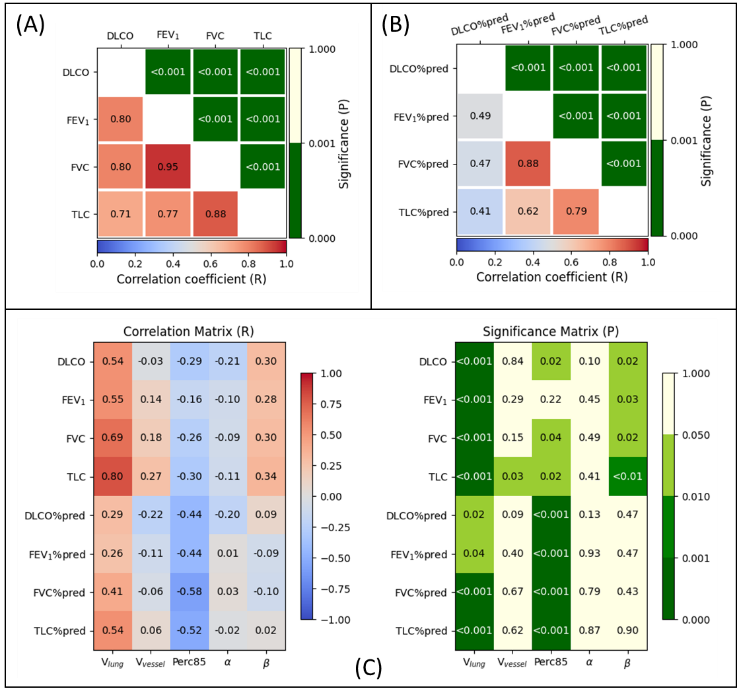
\includegraphics[width=8cm]{manual_biomarkers.png}
    \caption{Pearson correlation coefficients and corresponding significance levels: (A) between different absolute PFTs; (B) between different PFTs\%pred; and (C) between manually designed biomarkers and PFTs/PFTs\%pred, from the testing dataset.}
    \label{fig:chap4_manual}
\end{figure}



\subsection{Transfer learning (tl) versus trained from scratch (q2)}
 
The performance of the network based on TL was compared with the network trained from scratch, see Table \ref{chap4_table:table_TL}. It is shown that the R and ICC values increased and MAE values decreased after the introduction of TL. The standard deviation also decreased, which means that the networks with TL were more stable than those trained from scratch. This finding was verified by the scatter plots of the two networks (Figure \ref{fig:chap4_scatter}), where the regression lines of the network with TL were closer to the identity line than the networks without TL. Figure \ref{fig:chap4_ba} shows the Bland-Altman plots of networks without or with TL. The plots display the differences between the automatically estimated PFTs and measured PFTs against their mean. From Figure \ref{fig:chap4_scatter} and \ref{fig:chap4_ba}, we can observe that the network trained from scratch tended to give conservative estimations: close to the mean value of measurements.


% Please add the following required packages to your document preamble:
% \usepackage{multirow}
\begin{table}[tb]
\centering
\caption{Comparison between networks trained with or without transfer learning.  $^\dag$ Significance of the mean error difference between the networks with or without TL. $^\ddag$ Significance of the mean error difference between the 4-class and 1-class network. * Results of the four 1-class networks. }
\begin{tabular}{c|c|c|c|c|c|c}
\hline
\begin{tabular}[c]{@{}c@{}}Transfer\\ learning\end{tabular} & \begin{tabular}[c]{@{}c@{}}Network\\ type\end{tabular} & Metrics   & DLCOc    & FEV\textsubscript{1}     & FVC      & TLC      \\ \hline
\multirow{4}{*}{No}                                         & \multirow{4}{*}{4-class}                               & R         & 0.54     & 0.62     & 0.68     & 0.71     \\
                                                            &                                                        & ICC       & 0.48     & 0.58     & 0.65     & 0.70     \\
                                                            &                                                        & MAE       & 1.25     & 0.46     & 0.56     & 0.70     \\
                                                            &                                                        & MAPE      & 26\%     & 19\%     & 17\%     & 15\%     \\ \hline
\multirow{10}{*}{Yes}                                       & \multirow{5}{*}{4-class}                               & R         & 0.71     & 0.77     & 0.83     & 0.82     \\
                                                            &                                                        & ICC       & 0.71     & 0.76     & 0.8      & 0.81     \\
                                                            &                                                        & MAE       & 1.04     & 0.41     & 0.49     & 0.63     \\
                                                            &                                                        & MAPE      & 22\%     & 18\%     & 16\%     & 13\%     \\
                                                            &                                                        & $p-value^\dag$  & $<0.001$ & $<0.001$ & $<0.001$ & $<0.001$ \\ \cline{2-7} 
                                                            & \multirow{5}{*}{1-class}                               & R         & 0.71     & 0.76     & 0.78     & 0.85     \\
                                                            &                                                        & ICC       & 0.70     & 0.76     & 0.76     & 0.84     \\
                                                            &                                                        & MAE       & 1.07     & 0.38     & 0.51     & 0.55     \\
                                                            &                                                        & MAPE      & 23\%     & 16\%     & 17\%     & 12\%     \\
                                                            &                                                        & $p-value^\ddag$ & 0.60     & 0.13     & 0.18     & 0.61     \\ \hline
\end{tabular}

\label{chap4_table:table_TL}
\end{table}


Therefore, the images with lower PFTs were overestimated and higher PFTs were underestimated. After the introduction of TL, these pattern disappeared in FEV\textsubscript{1}, FVC and TLC, whereas in DLCO a similar but less prominent pattern remained. This indicates that the network trained with TL achieves a better agreement to measured PFTs. In addition, Figure \ref{fig:chap4_lr} shows that TL could speed up the training: decreasing the training epochs from 68 to 14. Therefore, we used TL in all the following experiments. 

\begin{figure}[tb]
    \centering
    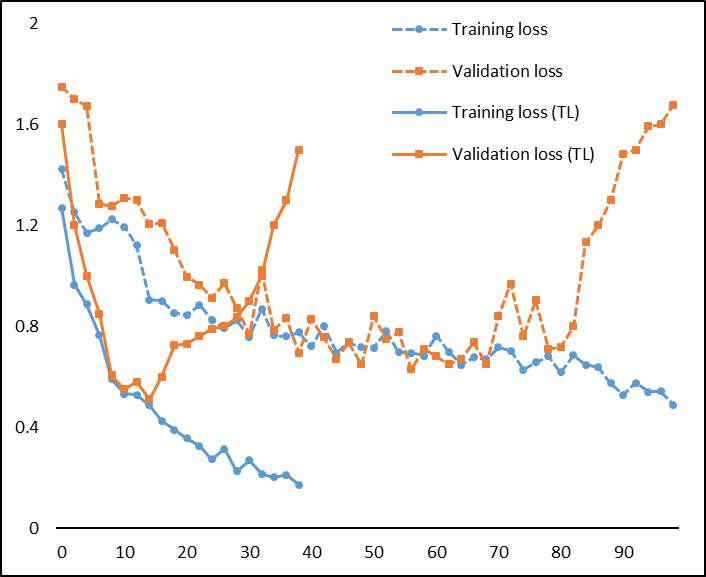
\includegraphics[width=8cm]{learning_curve.png}
    \caption{Comparison of training and validation curves with or without transfer learning (TL) on the same fold.}
    \label{fig:chap4_lr}
\end{figure}


\begin{figure}[tb]
    \centering
    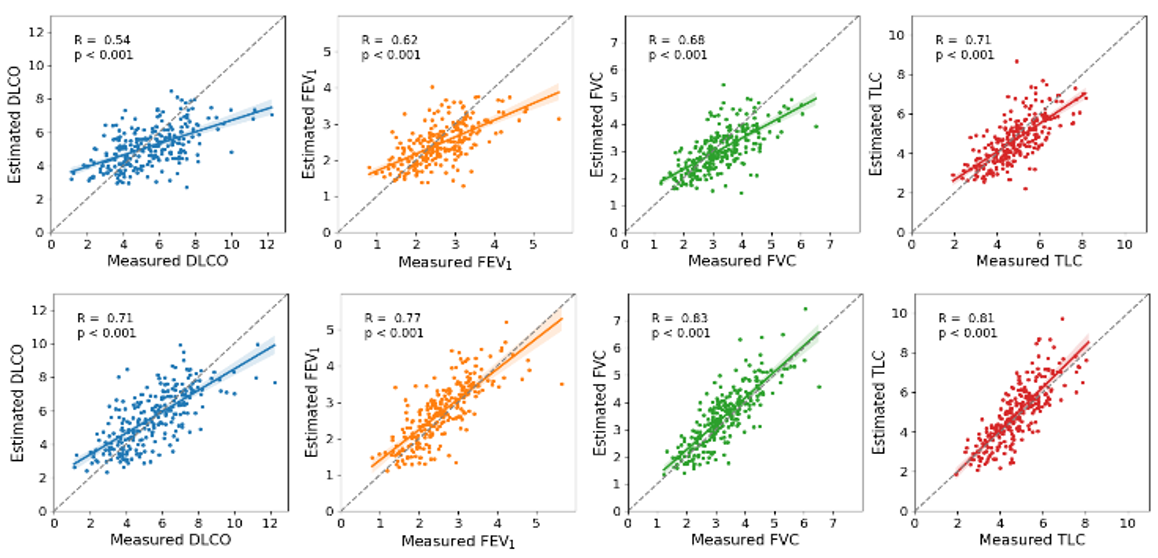
\includegraphics[width=8cm]{scatter.png}
    \caption{Scatter plots comparison between networks without (upper) and with (lower) transfer learning. Each image shows the identify line (dot line), regression line (solid line) and the 95\% confidence intervals (shaded areas).}
    \label{fig:chap4_scatter}
\end{figure}


\begin{figure}[tb]
    \centering
    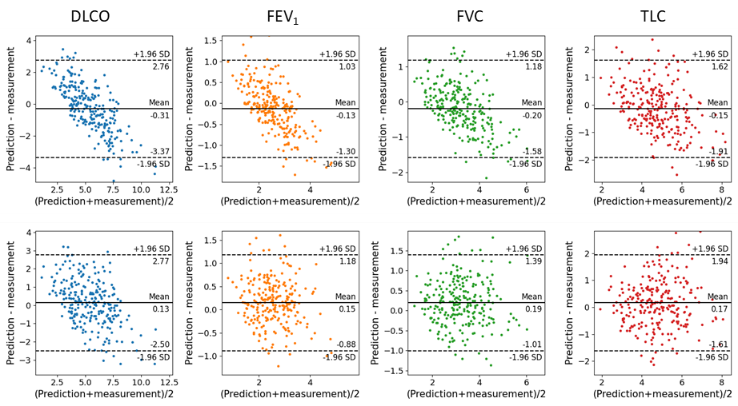
\includegraphics[width=8cm]{ba.png}
    \caption{Bland-Altman plots comparison between networks without (upper) and with (lower) transfer learning. The mean difference and the limits of agreement (mean ± 1.96 × SD, where SD is the standard deviation of the differences) are also shown on the plots.}
    \label{fig:chap4_ba}
\end{figure}


\subsection{Estimation of PFTs\%pred: direct versus indirect (q3)}

Table \ref{chap4_table:PFTpp} shows the performance of estimating PFTs\%pred for the two methods. The indirect estimation achieved ICC values of 0.60, 0.60, 0.69 and 0.75 for DLCO\%pred, FEV\textsubscript{1}\%pred, FVC\%pred and TLC\%pred, respectively. These ICC values were higher than those of the direct method (ICC=0.30, 0.47, 0.50 and 0.53). The indirect method also achieved higher R and lower MAE values. Therefore, all the following networks were trained to estimate the absolute PFTs first. 


% Please add the following required packages to your document preamble:
% \usepackage{multirow}
\begin{table}[tb]
\centering
\caption{PFT\% estimation comparison between two methods.The units of MAE are mL/min/mm Hg for DLCOc and liter for FEV\textsubscript{1}/FVC/TLC. }
\setlength{\tabcolsep}{1.8mm}{
\begin{tabular}{c|c|c|c|c|c}
\hline
Method  & Metrics & DLCOc\%     & FEV\textsubscript{1}\%      & FVC\%       & TLC\%       \\ 
\hline
\multirow{4}{*}{\begin{tabular}[c]{@{}c@{}}Direct    \end{tabular}}             
                & R       & 0.32        & 0.47        & 0.51        & 0.54        \\
                & ICC     & 0.30        & 0.47        & 0.50        & 0.53        \\
                & MAE & 17.30 & 14.88 & 14.98 & 13.59 \\ 
                 & MAPE & 29\% &	18\% &	18\% &	17\% \\ 
\hline
\multirow{4}{*}{\begin{tabular}[c]{@{}c@{}}Indirect\end{tabular}} 
                & R       & 0.60        & 0.65        & 0.74        & 0.76        \\
                & ICC     & 0.60        & 0.60        & 0.69        & 0.75        \\
                & MAE     & 13.85       & 14.79       & 13.76       & 11.04  \\ 
                & MAPE & 22\% &	18\% &	16\% &	13\%  \\ \hline
\end{tabular}}
\label{chap4_table:PFTpp}
\end{table}



\subsection{1-class versus 4-class (Q4)}

Table 2 shows that the ICC values of the 4-class network (ICC=0.71, 0.76, 0.80, and 0.81) were similar to the ICC values of tsshe four 1-class networks (ICC=0.70, 0.76, 0.76, and 0.84). The R and MAE values for the two network designs were also similar. \textit{p}-values of 0.60, 0.13, 0.18 and 0.61 indicate that the results of the four networks with 1-class output did not show a significantly difference compared to the 4-class network. Because the 4-class network can output four PFTs at a same time, which saves training \& inference time and GPU memory, all the following networks were trained with a 4-class output.

\subsection{Contribution of the different chest regions (q5)}
The PFT estimation performance of our proposed networks are summarized in Figure \ref{fig:chap4_bar} and Table \ref{chap4_table_all_compare}. DLCO was always the most difficult parameter to estimate, followed by FEV\textsubscript{1} and then FVC and TLC. The network trained on the whole CT volume achieved the best performance (highest ICC and R, as well as lowest MAE values). The network trained on both lungs performed slightly worse. The performances for the left and right lung were similar, which implies similar contribution of left and right lung to the PFT estimation. The network trained on pulmonary vessels performed worse than the previous networks for FEV\textsubscript{1}, FVC and TLC estimation, but better for DLCO estimation. The network trained on binarized vessels (1 as foreground and 0 as background) achieved similar ICC and MAE values and slightly higher R values, as compared to the network trained on gray scale vessels. The networks trained on gray scale vessels performed the worst compared to the other networks, but still better than the manually designed vessel based biomarkers $\alpha$ (R=-0.29) and $\beta$ (R=0.32).

\begin{figure}[tb]
    \centering
    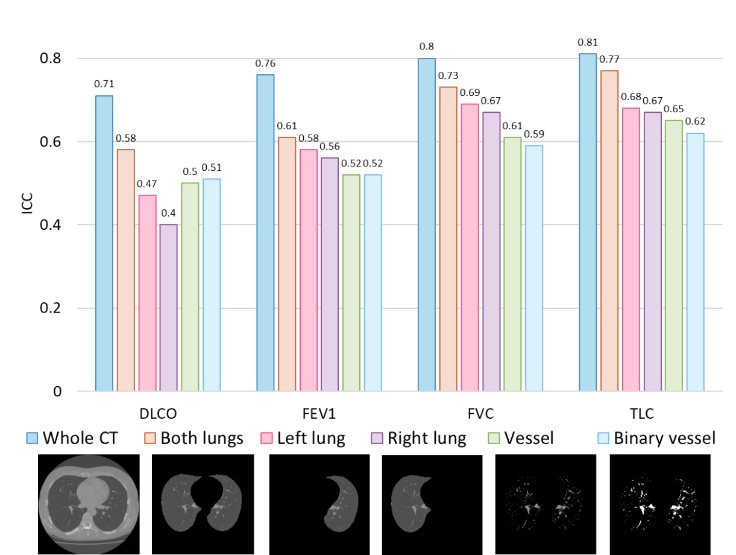
\includegraphics[width=8cm]{bar.png}
    \caption{Performance of the networks trained on different regions of the chest. The bars with different colors represent networks trained by different regions, which are illustrated at the bottom.}
    \label{fig:chap4_bar}
\end{figure}


% Please add the following required packages to your document preamble:
% \usepackage{multirow}
\begin{table}[tb]
\centering
\setlength{\tabcolsep}{1.8mm}{
\begin{tabular}{c|c|c|c|c|c}
\hline
Input                          & Metrics & DLCOc      & FEV\textsubscript{1}       & FVC         & TLC         \\ \hline
\multirow{3}{*}{Whole CT}      & R       & 0.71       & 0.77       & 0.83        & 0.82        \\
                               & MAE & 1.04  & 0.41  & 0.49   & 0.63   \\
                               & MAPE & 22\%  & 18\%  & 16\%   & 13\%   \\ \hline
\multirow{3}{*}{Both lungs}    & R       & 0.59       & 0.62       & 0.73        & 0.78        \\
                               & MAE & 1.19  & 0.45  & 0.49   & 0.57   \\
                               & MAPE & 27\%  & 20\%  & 16\%   & 13\%   \\ \hline
\multirow{3}{*}{Left lung}     & R       & 0.47       & 0.58       & 0.69        & 0.68        \\
                               & MAE & 1.29  & 0.48  & 0.56   & 0.74   \\
                               & MAPE & 28\% & 20\%  & 18\%   & 16\%   \\ \hline
\multirow{3}{*}{Right lung}    & R       & 0.45       & 0.59       & 0.69        & 0.69        \\
                               & MAE & 1.31  & 0.45  & 0.52   & 0.69   \\
                               & MAPE & 30\%   & 19\%   & 17\%   & 15\%   \\ \hline
\multirow{3}{*}{vessel}        & R       & 0.51       & 0.53       & 0.62        & 0.66        \\
                              & MAE & 1.28 & 0.53 & 0.58 & 0.74 \\
                               & MAPE & 27\%  & 23\%  & 19\%   & 16\% \\ \hline
\multirow{3}{*}{Binary vessel} & R       & 0.57       & 0.55       & 0.64        & 0.68        \\
                               & MAE & 1.28  & 0.52  & 0.62   & 0.76   \\
                               & MAPE & 27\%  & 22\%  & 19\%   & 16\%   \\ \hline
\end{tabular}
\caption{Performance of the networks trained from different inputs. The units of MAE are mL/min/mm Hg for DLCOc and liter for FEV\textsubscript{1}/FVC/TLC. DLCOc\%: DLCOc percent prediction; FEV\textsubscript{1}\%: FEV\textsubscript{1} percent prediction; FVC\%: FVC percent prediction; TLC\%: TLC percent prediction.}
\label{chap4_table_all_compare}
}
\end{table}


If we look at the RAMs generated from the network trained on whole CT, for some patients, the highlights are limited to the lungs, see Figure \ref{fig:chap4_ram} (left, row of Whole CT). For some other patients, the highlights also appeared outside the lungs (i.e. in the chest wall), see Figure \ref{fig:chap4_ram} (right, row of Whole CT). For all networks, the two center regions of the two lungs, where the larger pulmonary vessels are located, were highlighted the most. This pattern applied to the RAMs of all networks. The coronal views of RAMs were vertically  discontinuous; this is because the X3D-M network only applied pooling layers along the x and y axes, while leaving the z axis free of pooling layers, before the layer where our RAM\_3D was applied. That led to a narrow reception field along the z axis. 


\begin{figure}[tb]
    \centering
    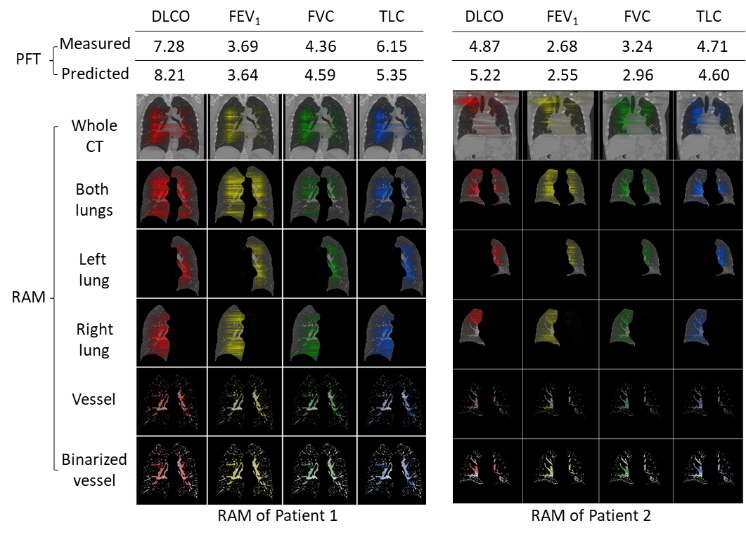
\includegraphics[width=8cm]{ram.png}
    \caption{Performance of the networks trained on different regions of the chest. The bars with different colors represent networks trained by different regions, which are illustrated at the bottom.}
    \label{fig:chap4_ram}
\end{figure}


\subsection{Comparison standard repeatability criteria (q6)}
After comparing our method to previous works, putting the results of our network into clinical perspective is still needed. Estimating PFTs from CT scans by human experts is impractical for obvious reasons, therefore we could not compare our method with human observations. However, we could compare our results with the theoretically best obtainable result, as determined by the officially recommended repeatability criteria for spirometric measurements. The PFT measures are normally obtained by means of three repetitions of the measurements \cite{Sylvester2020}. According to the most recent official standard on pulmonary function testing \cite{Sylvester2020}, the repeatability for DLCO and TLC obtained by the helium dilution technique between technically acceptable measurements should be within 10\% of the average value. The repeatability criterion for FEV1 and FVC is that differences should be lower than 0.15 L \cite{Sylvester2020}. To have a fair comparison between different PFTs, the acceptable errors of 0.15 L for FEV1 and FVC were divided by the mean measured values in Table \ref{chap4_table: dataset}, obtaining a percentage error of 6\% ($RE_{FEV_1} = 0.15/\bar{y}_{FEV_1} = 0.15/2.62 \approx 6\%$) and 5\% ($RE_{FVC} = 0.15/\bar{y}_{FVC} = 0.15/3.32 \approx 5\%$). As shown in Table \ref{chap4_table_compare_repeatibility}, the repeatability criteria is 10\%, 6\%, 5\% and 10\% for DLCO, FEV\textsubscript{1}, FVC and TLC, respectively. 

\begin{table}[h]
\centering
\caption{Comparison between official repeatability criteria and the relative error of our method.}
\begin{tabular}{c|c|c|c|c}
\hline
                                & DLCOc (\%) & FEV\textsubscript{1} (\%) & FVC (\%) & TLC (\%) \\ \hline
Repeatability criteria & 10         & 6         & 5        & 10       \\
Our model          & 20 ± 18    & 19 ± 14   & 15 ± 12  & 13 ± 11  \\
 \hline
\end{tabular}
\label{chap4_table_compare_repeatibility}
\end{table}




\subsection{Multiple variable regression analysis (q7)}
A multivariable regression analysis was performed to evaluate if manual biomarkers could still contribute to the estimation of PFTs, in addition to the estimation of our method. Multivariable stepwise linear regression was performed with DLCO as the dependent variable and the network-estimated DLCO (NetDLCO), Perc85, $\alpha$, $\beta$, $V\textsubscript{lung}$, and $V\textsubscript{vessel}$ as independent variables. We performed similar analyses for FEV\textsubscript{1}, FVC and TLC (Table \ref{chap4_table_multiple_variable}). The multivariable stepwise regression analysis showed that the inclusion of $V\textsubscript{lung}$ and $\beta$ could significantly improve the regression coefficient of DLCO (from R =0.75 to R =0.81). Similarly, by including $V\textsubscript{lung}$ and Perc85, the estimation of FEV\textsubscript{1}, FVC and TLC could also be significantly improved. Therefore, although we have developed automatic networks that outperformed manually designed biomarkers as single predictors, these manual biomarkers could still contribute further to the estimation of PFTs.

\begin{table}[]
\centering
\caption{Multivariable stepwise linear regressioin analysis for DLCOc, FEV\textsubscript{1}, FVC and TLC.}
% \setlength{\tabcolsep}{0.2mm}{
\begin{tabular}{lcllc}
\cline{1-2} \cline{4-5}
\multicolumn{2}{c}{\textbf{DLCOc}} &  & \multicolumn{2}{c}{\textbf{FEV\textsubscript{1}}} \\ \cline{1-2} \cline{4-5} 
Parameter                                & R                      &  & Parameter                                & R                     \\ \cline{1-2} \cline{4-5} 
NetDLCOc                                 & 0.750                  &  & NetFEV1                                  & 0.741                 \\
NetDLCOc+Lung-V                           & 0.781                  &  & NetDLCOc+Perc85                       & 0.828                 \\
NetDLCOc+Lung-V+$\beta$                      & 0.806                  &  &                                          &                       \\ \cline{1-2} \cline{4-5} 
                                         &                        &  &                                          &                       \\ \cline{1-2} \cline{4-5} 
\multicolumn{2}{c}{\textbf{FVC}}   &  & \multicolumn{2}{c}{\textbf{TLC}}  \\ \cline{1-2} \cline{4-5} 
Parameter                                & R                      &  & Parameter                                & R                     \\ \cline{1-2} \cline{4-5} 
NetFVC                                   & 0.823                  &  & NetTLC                                   & 0.686                 \\
NetFVC+Perc85                         & 0.868                  &  & NetTLC+Perc85                         & 0.766                 \\
NetFVC+Perc85+LungV                   & 0.877                  &  & NetDLCOc+Perc85+LungV                 & 0.807                 \\ \cline{1-2} \cline{4-5} 
\end{tabular}
\label{chap4_table_multiple_variable}
\end{table}

\section{Discussion and conclusion}
This paper demonstrated that it is feasible to automatically estimate comprehensive PFTs and PFTs\%pred from chest CTs, using deep learning. Our results indicate that CT scans can assist in estimating PFTs with considerable predictive accuracy. 

To the best of our knowledge, there is no currently published work on estimating PFT values for SSc patients. The only two works \cite{Park2023, choi2022automated} that aimed to automatically estimate PFTs from CT were developed based on 546 subjects diagnosed with lung cancer [5] or 16148 subjects with a risk of developing lung cancer \cite{Park2023}, as shown in Table 7. The R values of our method is slightly higher than Choi, et al. \cite{choi2022automated}, while the MAE of our method is higher than the other two works. Because we have already applied X3D with transfer learning, which achieved state-of-the-art performance on video recognition, possible reasons of the performance gap may include: 1) Dataset sizes are different. Considering the best MAE was achieved by the network trained on the largest number of subjects (16148 patients), there is still potential benefit from increasing the training set size for our network. 2) Different disease has different pathogenesis, leading to different difficulties in learning the relation between function and structure. In SSc patients, for example FVC may remain stable while DLCO significantly decline over time \cite{LeGouellec2017}. Therefore, compared with previous work, which only estimate FVC and FEV1, our work estimates a more comprehensive set of PFT measurements (DLCO, FEV1, FVC and TLC) for SSc patients, rendering it more clinically relevant for SSC patients, that is likely of additional clinical value. The comparison is for reference only, since it is based on different datasets sizes, different networks and different diseases. Implementing the two methods on our dataset to have an absolute fair comparison is impractical because the other two methods did not have public available pre-trained weights as what we have for X3D from Kinetics dataset.

The observed correlation between $\alpha$, $\beta$ and PFT in our study differs from the original report \cite{Zhai2016}. This is because patients with lung fibrosis were excluded in the original report, whereas our dataset comprised 80\% CT images with various degrees of fibrosis. In patients with lung fibrosis, fibrotic areas led to over-segmentation of vessels, decreasing the correlation between the $\alpha$ and $\beta$ calculated and PFT.

Estimating TLC was consistently more successful than for the other three PFT measurements. The MAE and prediction uncertainty in percentage (represented by MAPE) of TLC are always lower than the others. This could be explained by the fact that lung volume calculated by simply counting the number of voxels in both lungs is already strongly correlated with TLC, as measured by spirometry [29]. The estimation of DLCO consistently underperformed compared to the other three measures, since gas exchange is less correlated with TLC.
While the agreement between estimated PFTs and the measured PFTs ranged from moderate to good, the agreement between directly estimated PFTs\%pred and measured PFT\%pred ranged from poor to moderate. This finding is consistent with a previous report \cite{Park2023}. This can be attributed to the challenge of estimating reference equations for diverse population groups. Therefore we proceeded our research on estimating absolute PFTs, because 1) estimating PFTs\%pred indirectly was more accurate than a direct estimation; and 2) this approach is more flexible as other PFT biomarkers, such as FEV1/FVC \cite{Behr2008} and FVC/DLCO \cite{vallejos2020association}, can then also be derived from the estimated absolute PFT values.

From the comparison between networks trained by different regions of CT scans, we found that networks trained on the whole CT image could achieve the best performance. CT masked by both lungs produced slightly inferior results, suggesting that tissue outside the lung area still contribute to the estimation of PFTs to some extent. This observation could be verified by Figure 8, where some regions outside lungs are highlighted for Patient 2 in the first row (network trained on the whole CT) while regions outside lungs are not highlighted for Patient 1. This suggests that the interaction between the chest wall and intercostal muscles  contribute to PFTs in some patients. This is consistent with the clinical knowledge that stronger intercostal muscles combined with a compliant chest wall will have a positive effect on PFTs \cite{Park2020}. In contrast, chest wall stiffness, as sometimes observed in patients with SSc, may negatively influence PFTs. RAMs of different networks trained on different regions of CT have similar patterns: the entire lung is highlighted to different extents while the center regions of lungs are highlighted mostly. This implies that the networks for estimating PFTs need global information of the whole CT, while focusing more on the center regions where the largest vessels are located. This is consistent with findings in the previous study \cite{Park2023}. Apparently, it would be of greater clinical value if we could further extract what the contributors are. However, limited by the low resolution of current RAM techniques, we could not give more detailed contributors. Because a visualization centered on model interpretability would bridge the divide between AI-driven analyses and clinical practitioners, we will research more detailed visualization methods in our future work.

It is surprising that networks trained solely on grayscale vessels or binarized vessel masks still achieved R and ICC values over 0.5 for all four PFT measures. This implies that, in addition to vessel radius histogram information (used by $\alpha$ and $\beta$), the spatial structure of the vascular tree plays a more significant role in estimating PFTs.

Currently, there are no established guidelines for the level of precision required to implement new techniques in clinical practice for predicting PFTs. The repeatability criteria to measure PFTs is the standard for spirometry, which is the upper limit of any methods which aim to replace spirometry. At the current stage, our method could not perform competitively with spirometry if we compare our MAE with the repeatability criteria of spirometry. In addition, our method has not been prospectively validated, so it can only be used in research at present. Nevertheless, our method still 1) verified the possibility to estimate PFT, especially DLCO, from CT scans for patients of systemic sclerosis. 2) paved the way for more accurate methods and foster medical community to establish standards and regulations for such methods in the future. It would be beneficial to witness its integration into the clinical (randomized) trials in the future.

The multiple variable regression analysis showed that previous manually designed biomarkers could further explain variation in PFTs. This observation implies that if we add manually designed biomarkers as extra input to the networks, we might improve networks further in future research.

There are some limitations to our research. Because of the lack of public available 3D network weights pre-trained by lung CT images, we applied TL from Kinetics dataset, which may not optimal for PFTs estimation. In the future, we will explore the potential of network weights pre-trained from lung CT scans once we have the access to large annotated lung CT datasets. In addition, due to the need to protect healthy individuals from radiation exposure, it is not feasible to design a prospective experiment to collect CT and PFT pairs for a healthy control group. As a result, the retrospectively collected CT-PFT pairs in our study do not include healthy participants. Consequently, it remains uncertain whether our trained network can be applied to distinguish lung-structure relations in SSc patients from those in healthy individuals. Moreover, all SSc patients in this study were scanned with the same scanner at the same center. Therefore, additional experiments involving other patients and scanners are necessary to verify the generalizability of our deep learning method in the future. To achieve optimal performance for new scanners, we may need to fine-tune our model based on new datasets. If more image modalities are available in the future, we can explore the potential scalability of our methods on other modalities. Therefore, external validation is needed to be imbedded in clinical (randomized) trials. For now, the method can only be used for clinical research.

In conclusion, our method can automatically and comprehensively estimate PFTs for SSc patients. This can help to estimate lung function for patients who are unable to perform these tests, while there are CT scans available. The method can form a basis for studying the relation between function and structure, since we found for example that regions outside the lungs also contribute to the estimation of PFTs. For future work, we will investigate how to extract the contributors outside the lungs in more detail, which would be of great clinical value.

\section*{Acknowledgement}
This work is supported by the China Scholarship Council No.202007720110. This work was performed using the computational resources from the Academic Leiden Interdisciplinary Cluster Environment (ALICE) provided by the Leiden University.



